\NeedsTeXFormat{LaTeX2e}[2005/12/01]
%%    2009/03/12 v1.0 GAUBM Vorlage fuer Abschlussarbeiten Physik
%% Template fuer Bachelor- und Masterarbeiten
%% an der Fakultaet fuer Physik (c) Thomas Pruschke der GA Universitaet
%% Verbesserungsvorschlaege bitte an pruschke@theorie.physik.uni-goettingen.de
%%
%% Benoetigte Pakete: datenumber
%%

%%%%%%%%%%%%%%%%%%%%%%%%%%%%%%%%%%%%%%%%%%%%%%%%%%%%%%%%%%%%%%%%%%%%%%
%%%%%%%%%% Bitte vor dem Veraendern diese Datei umbenennen! %%%%%%%%%%
%%%%%%%%%%%%%%%%%%%%%%%%%%%%%%%%%%%%%%%%%%%%%%%%%%%%%%%%%%%%%%%%%%%%%%

%% scrbook - Ersatz fuerr LaTeX book Klasse aus dem KOMA Script
%% Moegliche Optionen: diejenigen der Klasse scrbook ausser titlepage
%% Updates, Fixes und Modifikationen von Boris Lemmer, 07.01.2015

%% deutsche Arbeit:
\documentclass[bachelor,       %% Typ der Arbeit: bachelor oder master
               twoside,        %% zweiseitiges Layout
               BCOR10mm,       %% Bindekorrektur 10 mm
%               liststotoc,nomtotoc,bibtotoc, %% Aufnahme der div. Verzeichnisse
                                              %% ins Inhaltsverzeichnis
              english,ngerman, %% Alternativspr. Englisch, Dokumentspr. Deutsch
%               ngerman,english  %% Alternativspr. Deutsch, Dokumentspr. Englisch
%               final,          %% Endversion; draft fuer schnelles Kompilieren
               ]{GAUBM}

\usepackage{setspace}  %% Zur Setzung des Zeilenabstandes
\usepackage{babel}     %% Sprachen-Unterstuetzung
\usepackage{calc}      %% ermoeglicht Rechnen mit Laengen und Zaehlern
\usepackage[T1]{fontenc}       %% Unterstutzung von Umlauten etc.
%\usepackage[latin1]{inputenc}  %% 
%% in aktuellem Linux & MacOS X wird standardmaessig UTF8 kodiert!
\usepackage[utf8]{inputenc}    %% Wenn latin1 nicht geht ...
\usepackage{color}
\usepackage{amsmath,amssymb} %% zusaetzliche Mathe-Symbole

\usepackage{lmodern} %% type1-taugliche CM-Schrift als Variante zur
                     %% "normalen" EC-Schrift
%% Paket fuer bibtex-Datenbanken
\usepackage[comma,numbers,sort&compress]{natbib}
%% modified by A.Quadt, 01.09.2010
% \bibliographystyle{plainnat}
\bibliographystyle{bthesis}
% added by A.Quadt, 01.09.2010
%\documentclass[11pt, a4paper, headsepline, footsepline]{scrbook}

\usepackage[latin1]{inputenc}
\usepackage{longtable}
\usepackage[it, bf]{caption}
\usepackage[dvips]{graphicx}
\usepackage{amsfonts}
\usepackage{amsmath}
\usepackage{mathrsfs}
\usepackage{epsfig}
\usepackage[clearempty]{titlesec}
\usepackage{booktabs}
\usepackage{hhline}
\usepackage{array}
\usepackage{subfigure}
%\usepackage{floatflt}
\usepackage{graphicx}% Include figure files
\usepackage{dcolumn}% Align table columns on decimal point
\usepackage{bm}% bold math
\usepackage{mathrsfs} 
\usepackage{amssymb}

% added by A.Quadt, 07.09.2010
\usepackage{amsfonts}
\usepackage{amsmath}
\usepackage{mathrsfs}
\usepackage{xspace}
%

\setlength{\oddsidemargin}{0cm}
\setlength{\evensidemargin}{0cm}
\setlength{\topmargin}{-1cm}
\setlength{\textheight}{23cm}
\setlength{\textwidth}{16cm}

\pagestyle{headings}

\renewcommand{\sectfont}{\bfseries\rmfamily}
\renewcommand{\floatpagefraction}{0.7}
\renewcommand{\textfraction}{0.1}

% abbreviations added, A.Quadt, 07.09.2010
%
\newcommand{\dzero}      {D\O\xspace}
\newcommand{\cdf}        {CDF\xspace}
\newcommand{\uubar}      {\mbox{$u\bar{u}$}}
\newcommand{\ddbar}      {\mbox{$d\bar{d}$}}
\newcommand{\ccbar}      {\mbox{$c\bar{c}$}}
\newcommand{\ssbar}      {\mbox{$s\bar{s}$}}
\newcommand{\ttbar}      {\mbox{$t\bar{t}$}}
\newcommand{\bbbar}      {\mbox{$b\bar{b}$}}
\newcommand{\wjets}      {\mbox{$W + 4\; jets$}}
\newcommand{\pttbar}     {\mbox{$p_{t\bar{t}}$}}
\newcommand{\pwjets}     {\mbox{$p_{W +4 \; jets}$}}
\newcommand{\ljets}      {\mbox{$\ell + \; jets$}}
\newcommand{\ejets}      {\mbox{$e + \; jets$}}
\newcommand{\mujets}     {\mbox{$\mu + \; jets$}}
%
%
\newcommand{\fermilab}  {{F{\sc ermilab}}\xspace}
\newcommand{\tevatron}  {{T{\sc evatron}}\xspace}
\newcommand{\opal}      {{O{\sc pal}}\xspace}
\newcommand{\cern}      {{C{\sc ern}}\xspace}
\newcommand{\fnal}      {{F{\sc nal}}\xspace}
\newcommand{\atlas}     {{A{\sc tlas}}\xspace}
\newcommand{\lhc}       {{L{\sc hc}}\xspace}
\newcommand{\lep}       {{L{\sc ep}}\xspace}
\newcommand{\slc}       {{S{\sc lc}}\xspace}
\newcommand{\pep}       {{P{\sc ep}}\xspace}
\newcommand{\petra}     {{P{\sc etra}}\xspace}
\newcommand{\hera}      {{H{\sc era}}\xspace}
\newcommand{\lepaleph}  {{A{\sc leph}}\xspace}
\newcommand{\delphi}    {{D{\sc elphi}}\xspace}
\newcommand{\leplthree} {{L{\sc 3}}\xspace}
\newcommand{\lepopal}   {{O{\sc pal}}\xspace}
\newcommand{\doris}     {{D{\sc oris}}\xspace}
\newcommand{\isr}       {{I{\sc sr}}\xspace}
\newcommand{\desy}      {{D{\sc esy}}\xspace}
\newcommand{\kek}       {{K{\sc ek}}\xspace}
\newcommand{\slac}      {{S{\sc lac}}\xspace}
\newcommand{\tristan}   {{T{\sc ristan}}\xspace}
\newcommand{\cms}       {{C{\sc ms}}\xspace}
\newcommand{\alice}     {{A{\sc lice}}\xspace}
\newcommand{\zeus}      {{Z{\sc eus}}\xspace}
\newcommand{\hone}      {{H{\sc 1}}\xspace}
\newcommand{\minuit}    {{M{\sc inuit}}\xspace}
\newcommand{\herwig}    {{H\sc{erwig}}\xspace}
\newcommand{\acermc}    {{A\sc{cerMC}}\xspace}
\newcommand{\evtgen}    {{E\sc{vtgen}}\xspace}
\newcommand{\mcfm}      {{M\sc{cfm}}\xspace}
\newcommand{\mcatnlo}   {{M\sc{c@nlo}}\xspace}
\newcommand{\sherpa}    {{S\sc{herpa}}\xspace}
\newcommand{\jimmy}     {{J\sc{immy}}\xspace}
\newcommand{\cteq}      {{C\sc{teq}}\xspace}
\newcommand{\pythia}    {{P\sc{ythia}}\xspace}
\newcommand{\jetnet}    {{J\sc{etnet}}\xspace}
\newcommand{\isajet}    {{I\sc{sajet}}\xspace}
\newcommand{\jetset}    {{J\sc{etset}}\xspace}
\newcommand{\vecbos}    {{V\sc{ecbos}}\xspace}
\newcommand{\alpgen}    {{A\sc{lpgen}}\xspace}
\newcommand{\vegas}     {{V\sc{egas}}\xspace}
\newcommand{\gnu}       {{G\sc{nu}}\xspace}
\newcommand{\onetop}    {{O\sc{neTop}}\xspace}
\newcommand{\ztop}      {{Z\sc{Top}}\xspace}
\newcommand{\toprex}    {{T\sc{opRex}}\xspace}
\newcommand{\singletop} {{S\sc{ingleTop}}\xspace}
\newcommand{\madgraph}  {{M\sc{adgraph}}\xspace}
\newcommand{\madevent}  {{M\sc{adevent}}\xspace}
\newcommand{\comphep}   {{C\sc{omphep}}\xspace}
\newcommand{\qq}        {{Q\sc{q}}\xspace}
\newcommand{\tauola}    {{T\sc{auola}}\xspace}
\newcommand{\geant}     {{G\sc{eant}}\xspace}
\newcommand{\GEANT}     {{G\sc{eant}}\xspace}
\newcommand{\amegic}    {{A\sc{megic++}}\xspace}

\newcommand{\met}       {\mbox{$\not\!\!E_T$}\xspace}
\newcommand{\metcal}    {\mbox{$\not\!\!E_{Tcal}$}\xspace}
\newcommand{\MET}       {$\not\!\!E_T$}
\newcommand{\lowmet}    {low-\mbox{$\not\!\!E_T$}-QCD\xspace}

\newcommand{\runi}      {Run~I\xspace}
\newcommand{\runii}     {Run~II\xspace}

%\newcommand{\dzero}      {D\O}
%\newcommand{\uubar}      {\mbox{$u\bar{u}$}}
%\newcommand{\ddbar}      {\mbox{$d\bar{d}$}}
%\newcommand{\ccbar}      {\mbox{$c\bar{c}$}}
%\newcommand{\ssbar}      {\mbox{$s\bar{s}$}}
%\newcommand{\ttbar}      {\mbox{$t\bar{t}$}}
%\newcommand{\bbbar}      {\mbox{$b\bar{b}$}}
%\newcommand{\wjets}      {\mbox{$W + 4\; jets$}}
%\newcommand{\pttbar}     {\mbox{$p_{t\bar{t}}$}}
%\newcommand{\pwjets}     {\mbox{$p_{W +4 \; jets}$}}
%\newcommand{\ljets}      {\mbox{$l + \; jets$}}
%\newcommand{\ejets}      {\mbox{$e + \; jets$}}
%\newcommand{\mujets}     {\mbox{$\mu + \; jets$}}
%\newcommand{\herwig}     {{\sc herwig}}



\newcommand{\tabheadfont}[1]{\textbf{#1}} %% Tabellenkopf in Fett
\usepackage{booktabs}                      %% Befehle fuer besseres Tabellenlayout
\usepackage{longtable}                     %% umbrechbare Tabellen
\usepackage{array}                         %% zusaetzliche Spaltenoptionen

%% umfangreiche Pakete fuer Symbole wie \micro, \ohm, \degree, \celsius etc.
\usepackage{textcomp,gensymb}

%\usepackage{SIunits} %% Korrektes Setzen von Einheiten
\usepackage{units}   %% Variante fuer Einheiten

%% Hyperlinks im Dokument; muss als eines der letzten Pakete geladen werden
\usepackage[pdfstartview=FitH,      % Oeffnen mit fit width
            breaklinks=true,        % Umbrueche in Links, nur bei pdflatex default
            bookmarksopen=true,     % aufgeklappte Bookmarks
            bookmarksnumbered=true  % Kapitelnummerierung in bookmarks
            ]{hyperref}
%---------------
% Selbst definierte Befehle
%---------------
\newcommand{\comment}[1]{{\textit{\color{red} #1}}}  

%% Weiter benoetigte Pakete: datenumber
%% Falls dieses Paket nicht in der Installation vorhanden ist,
%% kann es von der Seite mit diesem Template heruntergeladen werden
%% und in einem LaTeX bekanntem Verzeichnis installiert werden (notfalls
%% dem Verzeichnis mit der Arbeit).
\begin{document}
%%
%%                   Ab hier muessen die Anpassungen geschehen
%%
%% Hier den eigenen Namen einsetzen
\ThesisAuthor{Philip}{Marszal}
%% Hier den Geburtsort einsetzen
\PlaceOfBirth{Kassel}
%% Titel Arbeit. Das erste Argument ist der deutsche, das zweite der
%% englische Titel.
\ThesisTitle{Spezialisierungspraktikum in der Kern- und Teilchenphysik}{}
%% Erst- und Zweitgutacher/in
%% Ist der/die Betreuer/in nicht identisch mit dem/r Erstgutachter/in,
%% muss diese/r als optionales Argument angegeben werden.
%% Diese Angaben beziehen sich auf Institut-externe BetreuerInnen und sollten nur in Ausnahmen relevant sein.
%%\FirstReferee[Dr.\ \ldots]{Prof.\ Dr.\ \dots} % fuer externe Betreung
\FirstReferee{Prof.\ Dr.\ Quadt}                % fuer interne Betreung
%% Optionen mit Stand 01. Januar 2014:
%% Prof.~Dr.~Ariane Frey
%% Priv.Doz.~Dr.~J{\"o}rn Gro{\ss}e-Knetter
%% Prof.~Dr.~Hans Hofs{\"a}ss
%% Prof.~Dr.~Arnulf Quadt
%% Jun.Prof.~ Steffen Schumann
\Institute{II. Physikalischen Institut}
\SecondReferee{Prof.\ Dr.\ \dots}
%% added by A.Quadt, 31.08.2010
%% Referenz Nummer der Bachelorarbeit im Institut
\ReferenceNumber{II.Physik-UniG{\"o}-BSc-2014/01}
%%
%% Beginn und Ende des Anfertigungszeitraumes
\ThesisBegin{2}{3}{2015}
\ThesisEnd{31}{3}{2015}
%% DO NOT TOUCH THESE LINES!!!!
\frontmatter
\maketitle
%% Ende des Vorspanns
\cleardoublepage
%% Ab hier 1 1/2 facher Zeilenabstand (durch setspace-Paket)
\onehalfspacing
%% Erzeugt Inhaltsverzeichnis
\tableofcontents

%% Hier kann man seine Bezeichnungsweisen erklaeren. Falls nicht
%% benoetigt, bis einschliesslich \end{nomenclature} auskommentieren
\begin{nomenclature}
%% Fuer die Berechnung der Spaltenbreiten muss \usepackage{calc}
%% geladen sein!
\section*{Lateinische Buchstaben}
\noindent
\begin{longtable}[l]{p{0.2\textwidth}p{0.7\textwidth-6\tabcolsep}p{0.1\textwidth}}
  \tabheadfont{Variable}&\tabheadfont{Bedeutung}&\tabheadfont{Einheit}\\\midrule\endhead
  $A$ & Querschnittsfl{\"a}che & $\unit{m^2}$\\
  $c$ & Geschwindigkeit & $\unitfrac{m}{s}$
\end{longtable}
\section*{Griechische Buchstaben}
\begin{longtable}[l]{p{0.2\textwidth}p{0.7\textwidth-6\tabcolsep}p{0.1\textwidth}}
  \tabheadfont{Variable}&\tabheadfont{Bedeutung}&\tabheadfont{Einheit}\\\midrule\endhead
  $\alpha$  & Winkel & $\unit{\degree}$; --\\
  $\varrho$ & Dichte & $\unitfrac{kg}{m^3}$
\end{longtable}
\section*{Indizes}
\begin{longtable}[l]{p{0.2\textwidth}p{0.8\textwidth-4\tabcolsep}}
  \tabheadfont{Index}&\tabheadfont{Bedeutung}\\\midrule\endhead
  m & Meridian\\
  $r$ & Radial
\end{longtable}
\section*{Abk{\"u}rzungen}
\begin{longtable}[l]{p{0.2\textwidth}p{0.8\textwidth-4\tabcolsep}}
  \tabheadfont{Abk"urzung}&\tabheadfont{Bedeutung}\\\midrule\endhead
  2D & zweidimensional\\
  3D & dreidimensional\\
  max & maximal
\end{longtable}
\end{nomenclature}
%% \listoftables und \listoffigures sollten nur bei genuegender Anzahl Tabellen
%% verwendet werden
%\listoffigures
%\listoftables

\mainmatter   %% Anfang Hauptteil

\chapter{Einleitung}
Um sich mit den komplexen Themen einer Bachelorarbeit im Bereich Teilchenphysik auseinandersetzen zu können, ist ein grundlegendes Verständnis der Theorie und experimentellen Methoden der Hochenergie-Physik notwendig. Im Verlauf des Spezialisierungspraktikums wurden Themen von den Anfängen der Quantenchromodynamik (QCD), über das Standartmodell, bis hin zu \'~Beyond the Standardmodel\'~ bearbeitet. Es wurde sich intensiv damit beschäftigt wie man Vorgänge der Teilchenphysik experimentell messen kann. Im letzten Teil des Spezialisierungspraktikums, wurden fundamentale Werkzeuge für die Analyse von experimentellen Daten aus Kollisionsexperimenten (insbesondere des \lhc am \cern) behandelt.  

\\
Tadda
\\
\chapter{Grundlagen}
\section{Das Standardmodell}
Das Standardmodell(SM) beschreibt alle bekannten Elementarteilchen und die zwischen ihnen herrschenden Wechselwirkungen. Die Elementarteilchen sind dabei in drei verschiedene Gruppen aufgeteilt: Quarks, Leptonen und Eichbosonen. Quarks und Leptonen sind Fermionen während Eichbosonen offensichtlich Bosonen sind. Die drei grundlegenen Wechselwirkungen, die durch das SM beschrieben werden sind: die elektromagnetische Wechselwirkung, die schwache Wechselwirkung und die starke Wechselwirkung. Die Gravitation wird jedoch nicht durch das SM beschrieben.
Jede Wechselwirkung verfügt über Austauschteilchen. Diese Teilchen sind die zur Kraft gehörenden Eichbosonen. Die Austauschteilchen der starken Wechselwirkung sind die Gluonen, die Austauschteilchen der elektromagnetischen Kraft sind die Photonen und die Austauschteilchen der schwachen Kraft sind die massiven $W^{\pm}$- und $Z^{0}$-Bosonen.
Die Fermionen des Standartmodells werden durch die Wechselwirkungen denen sie unterliegen charakterisiert. Neutrinos, die zu den Leptonen gehören, wechselwirken nur schwach, geladene Leptonen, wie z.B. das Elektron, wechselwirken schwach und elektromagnetisch. Quarks nehmen an jeder Wechselwirkung teil, insbesondere der starken Wechselwirkung.

\section{Quantenchromodynamik}
\subsection{Allgemeines}
Die Quantenchromodynamik ist die Theorie, die die starke Wechselwirkung beschreibt. Die Teilchen, die stark wechselwirken sind lediglich Quarks und Gluonen. So wie die elektromagnetische Kraft hat auch die starke Wechselwirkung eine Ladung, welche Farbe genannt wird. Es gibt dabei drei Farben: rot, grün und blau. Zusätzlich existieren noch die dazugehörigen Antifarben. 
\subsection{Regge-Theorie}
Die fühe Form der QCD ist die Regge-Theorie, die Vorgänge selbst bei nicht perturbativen Energien beschreiben kann. Der Kern der Regge-Theorie ist das Zulassen von komplexen Drehimpulsen bei Streuprozessen(Partialwellenansatz). Dabei werden sogenannte Trajektorien $\alpha(m^2)$ eingeführt, die den Drehimpuls in Abhängigkeit von der Energie darstellen. Die Energien an denen die Trajekorien ganzzahlige Werte annehmen entsprechen der Ruhemasse von Ausstauschteilchen mit entsprechendem Drehimpuls. Auf diese Weise kann man, wenn man den Drehimpuls und die Masse eines Teilchens kennt, eine Reihe weiterer Teilchen vorhersagen. Im Rahmen der Streutheorie werden aus den Trajektorien die Wirkungsquerschnitte errechnet\comment{Die Quelle ist: http://school-diff2013.physi.uni-heidelberg.de/Talks/Poghosyan.pdf ... Das ist eine Praesentation}: 
\begin{align*}
\sigma_{i} \propto \left(\frac{s}{s_0}\right)^{\alpha_i(0)-1}
\end{align*}
Betrachtet man alle bisher experimentell beobachteten Ausstauschteilchen für die Streuung, folgt dass der Wirkungsquerschnitt(WQS) mit steigender Schwerpunktsenergie $\sqrt{s}$ sinken müsste. Allerdings wird beobachtet, dass der WQS steigt. Dafür führt die Regge-Theorie das sogenannte \emph{Pomeron} ein. Die Trajektorie des Pomerons soll gerade den zuwachs des WQS erklären. Dieses Austauschteilchen lässt sich auf den Austausch von Gluonen bzw. Glueballs zurückführen. 
\subsection{Die starke Kopplundkonstante $\alpha_s$}
So wie die elektromagnetische Wechselwirkung, wird auch die Stärke der starken Wechselwirkung durch eine Kopplungskonstante bestimmt. Bei der elektromagnetischen Kraft wird eine theoretisch unendliche Ladung, durch Teilchen-Antiteilchen-Paare, die spontan entstehen und sich wieder vernichten, abgeschirmt. Dies führt zu dem Effekt, dass die Kopplungskonstante $\alpha_{em}$ bei steigenden Energien (d.h. geringerem Abstand zur Ladung) größer wird, weil weniger Abschirmung vorhanden ist. Dasselbe Phänomen gibt es bei der Farbladung. Jedoch wird die Abschirmung durch Quark-Antiquark-Paare von einer Verstärkung der Ladung durch Gluonen übertroffen. Aus diesem Effekt folgt die asympotische Freiheit der Quarks, die besagt dass die Kraft zwischen Quarks bei steigender Energie abnimmt. Auch Hadronisation hängt mit dem Verhalten der starken Wechselwirkung bei unterschiedlichen Energien zusammen.
\subsection{Partonen Verteilungen (PDF)}
Bei der Untersuchung von Hadron-Kollisionen ist es für die theoretische Behandlung nötig die Partonendichte innerhalb der Hadronen zu kennen, da diese sich direkt auf die Wirkungsquerschnitte der aller Reaktionen auswirkt. Gerade der Impuls der einzelnen Partonen spielt eine wichtige Rolle.

\section{Jet-Physik}
\subsection{Hadronisation}
Bei Kollisionen in Teilchenbeschleunigern wie dem \lhc am \cern, enstehen zunächst freie Quarks. Allerdings sind freie Quarks in der Natur nicht nachzuweisen, da die starke Kopplungskonstante, bei wachsendem Abstand zwischen zwei Teilchen mit Farbladung, wächst. Ein einzelnes Quark hätte demnach ein unendliches Potential. Das Phänomen, dass Quarks nicht einzeln vorkommen wird als \emph{Confinement} bezeichnet. Wenn nun bei einer Reaktion zwei Quarks entstehen, die entgegengesetzte Impulse haben bzw. sich auseinander bewegen, so steigt das Potential zwischen den Quarks an bis genug Energie im Potential ist um ein Quark-Antiquark-Paar zu erzeugen. Die beiden entstehenden Quarks bilden nun mit den beiden ursprünglichen Quarks stabile Hadronen. Dieser Prozess wird als Hadronisation bezeichnet. Aus einem einzelnen Quark entstehen dabei eine große Anzahl an Hadronen. Im Detektor werden deshalb Quarks als Hadronenschauer, auch Jets genannt, sichtbar. Beim Detektieren spielt das $b$-Quark eine besondere Rolle, da die Zeit, die das $b$-Quark zur Hadronisation braucht, im Vergleich zu allen anderen Quarks besonders lang ist und deshalb vom $b$-Quark stammende Jets ($b$-Jets) identifiziert werden können.
\subsection{Transversale Masse}
Mit der relativistischen Energie-Impuls-Beziehung lässt sich die Ruhemasse eines Teilchens aus seinem Vierer-Impuls $p^\mu$ berechnen. Auf diese Weise lässt sich aus zwei im Detektor gemessenen Teilchen die Ruhemasse des Mutterteilchens berechnen, da gelten muss:
\begin{align*}
M_{\text{Mutterteilchen}}^2 = p_\mu p^\mu = (p_{\text{Teilchen} 1}+p_{\text{Teilchen} 2})^2
\end{align*}
Versucht man jedoch auf diese Weise die Masse eines $W$-Bosons zu rekonstruieren trifft man auf Schwierigkeiten. Zerfällt ein $W$-Boson in ein geladenes Lepton und ein Neutrino, so kann man die die Vierevektoren nicht einfach addieren, da der Viererimpuls des Neutrinos nicht direkt gemessen werden kann, sondern nur anhand von Impulserhaltung rekonstruiert werden kann. Allerdings kann der Impuls in $z$-Richtung nicht rekonstruiert werden, da die im Beschleuniger kollidierenden Teilchen unterschiedliche Geschwindigkeiten in $z$-Richtung haben können. Deshalb wird in diesem Fall die transversale Masse definiert. Für die Masse des $W$-Bosons im $\ell \nu$-Kanal erhält man dann die folgende Formel:
\begin{align*}
M_W^T = \sqrt{2E_{\ell}^TE_\nu^T\left(1-\cos \Delta\Phi_{\ell,\nu}\right)}
\end{align*}
Dieser Wert hat eine obere Grenze bei der exakten Masse des $W$-Bosons.

\section{Top-Quark Physik}
\section{Vorhersage des Top-Quarks}
Aus Experimenten mit Kaonen wurde deutlich, dass die $CP$-Symmetrie verletzt ist. Die Eigenzustände eines Kaons zur $CP$-Symmetrie können als Superpositionen von Kaon und Antikaon beschrieben werden. Beide Zustände zerfallen in Pionen, wobei die Masse des Kaons nur geringfügig größer ist als die Masse von drei Pionen. Nun haben zwei Pionen einen $CP$-Eigenwert von $+1$ während eine ungerade Anzahl von Pionen einen Wert von $-1$ hat. Daraus folgt, dass das Kaon mit $CP=1$ schnell in zwei Pionen zerfällt, während
 das andere Kaon langsam in drei Pionen zerfällt. Im Experiment wurde nachgewiesen, dass selbst nach einer Zeit in der die kurzlebigen Kaonen zerfallen sein müssen, noch immer Kaonen in zwei Pionen zerfallen. Dies stellt eine Verletzung der $CP$-Symmetrie dar. Um diese $CP$-Brechung zu erklären muss eine komplexe Phase in die Elemente der CKM-Matrix eingeführt werden. Dies ist jedoch nur möglich wenn die Matrix mindestens eine Größe von $3\times 3$ hat. Deswegen ist eine dritte Generation von Quarks notwendig.
 
 \section{Entdeckung und Eigenschaften}
 \comment{Quellen sind vor allem PDG}Das Topquark wurde erstmals 1995 am \tevatron in den Detektoren \dzero und \cdf nachgewiesen. Mit einer Ruhemasse von $173.34 \pm 0.27(\text{stat.}) \pm 0.71 \text{sys.}$~GeV ist es das schwerste Elementarteilchen. Seine Zerfallsbreite ist $2.0\pm0.5$~GeV und seine Lebensdauer ist damit ca. $5\cdot10^{-25}$~s \comment{Bessere Quelle als Wikipedia finden!!!}. Diese geringe Lebensdauer liegt deutlich unter der Zeit die das Top-Quark zur Hadronisation brauchen würde. Damit ist es das einzige Quark, das zerfällt bevor es Hadronisieren kann. Dies macht es besonders leicht die Masse des Top-Quarks zu bestimmen.
 
 \section{Produktion von Top-Quarks}
 Die Produktion von Top-Quarks am \lep am \cern würde vorherrschend über Annihilation der Elektronen geschehen. Diese Annihilation kann über Photon oder $Z$-Boson stattfinden. Es ist in erster Ordnung nur möglich Top-Paare zu erzeugen, weswegen eine besonders hohe Schwerpunktsenergie notwendig wäre. Es wären ca. $340$~GeV nötig gewesen während die Höchstleistung des LEP bei $209$~GeV lag. Am \tevatron wurden hauptsächlich Top-Paare durch Annihilation zweier leichter Quarks erzeugt. Aufgrund der geringen Energie ($2$~TeV) rühren der Großteil der Reaktionen von Quark-Quark-Interaktionen her. Wechselwirkungen zwischen Gluonen spielen eine untergeordnete Rolle. Die Produktion von einzelnen Top-Quarks kann nur über die schwache Wechselwirkung stattfinden. Dazu muss allerings die Quark-Generation gewechselt werden, weswegen diese Reaktion unterdrückt ist. 
 Am \lhc werden Top-Quarks vor allem über Gluon-Gluon-Wechselwirkungen erzeugt. 

 \section{Higgs-Boson Physik}



\chapter{Detektorphysik}
\section{Teilchen in Materie}
\subsection{Bethe-Bloch}
Geladene Teilchen die sich durch Materie bewegen verlieren durch Interaktionen mit den Atomen an Energie. Diese Interaktionen umfassen Bremsstrahlung bei hohen Energien, Ionisation bei mittleren Energien und Anregung von Atomen bei geringen Energien. Der Energieverlust in Abhängigkeit von der Energie des Teilchens ist in Abb. \ref{fig:bethe} dargestellt.\comment{Rpp2012-rev-passage-particles-matter}Für schwere geladene Teilchen, wie z.B. das Muon wird der Energieverlust durch Ionisation durch die Bethe-Bloch Formel beschrieben.
\begin{align*}
- \left<\frac{dE}{dx}\right> =  K\cdot \frac{Z}{A}\frac{z^2}{\beta^2} \cdot \left[ \frac12\ln \left(\frac{2m_ec^2\cdot\beta^2\cdot\gamma^2 \cdot T_{max}}{I^2}\right) - \beta^2 - \frac{\delta(\beta\gamma)}{2}\right]
\end{align*} 
Diese Formel hängt lediglich von der Ladung $z$ und der relativistischen Geschwindigkeit $\beta$ des Teilchens und dem Material $K$ ab. Sie hängt explizit nicht von der Masse des Teilchens ab. Sie gibt den mittleren Energieverlust pro Strecke an. 
\begin{figure}
\centering
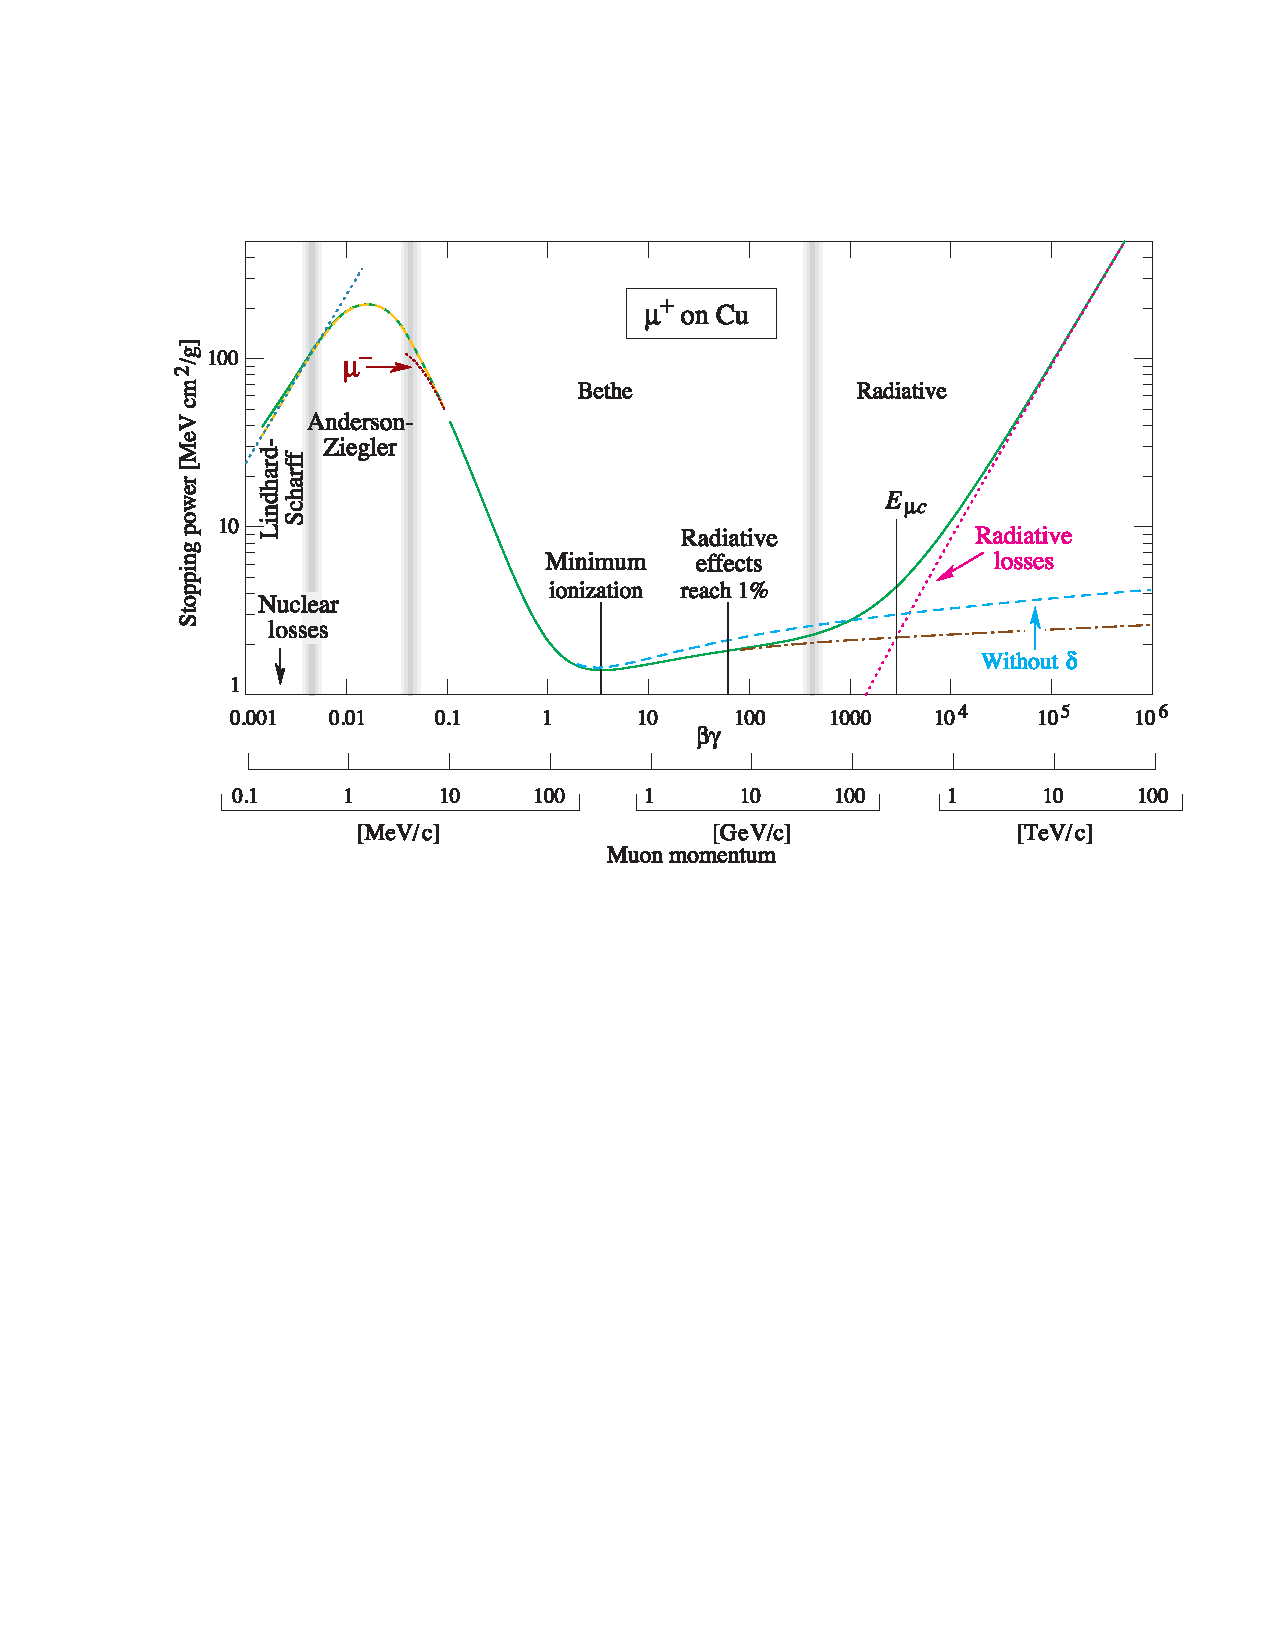
\includegraphics[scale=0.7]{./input/bethe.pdf}\caption{Energieverlust pro Strecke (Stopping power) aufgetragen gegen den Impuls eines Muons. Der Verlust durch Ionisation findet in einem Bereich von 10~Mev und 100~GeV statt\cite{Passage_through_matter}.}\label{fig:bethe}
\end{figure}
Um diesen Mittelwert ist der Energieverlust nach der Landau-Verteilung verteilt.
\begin{figure}
\centering
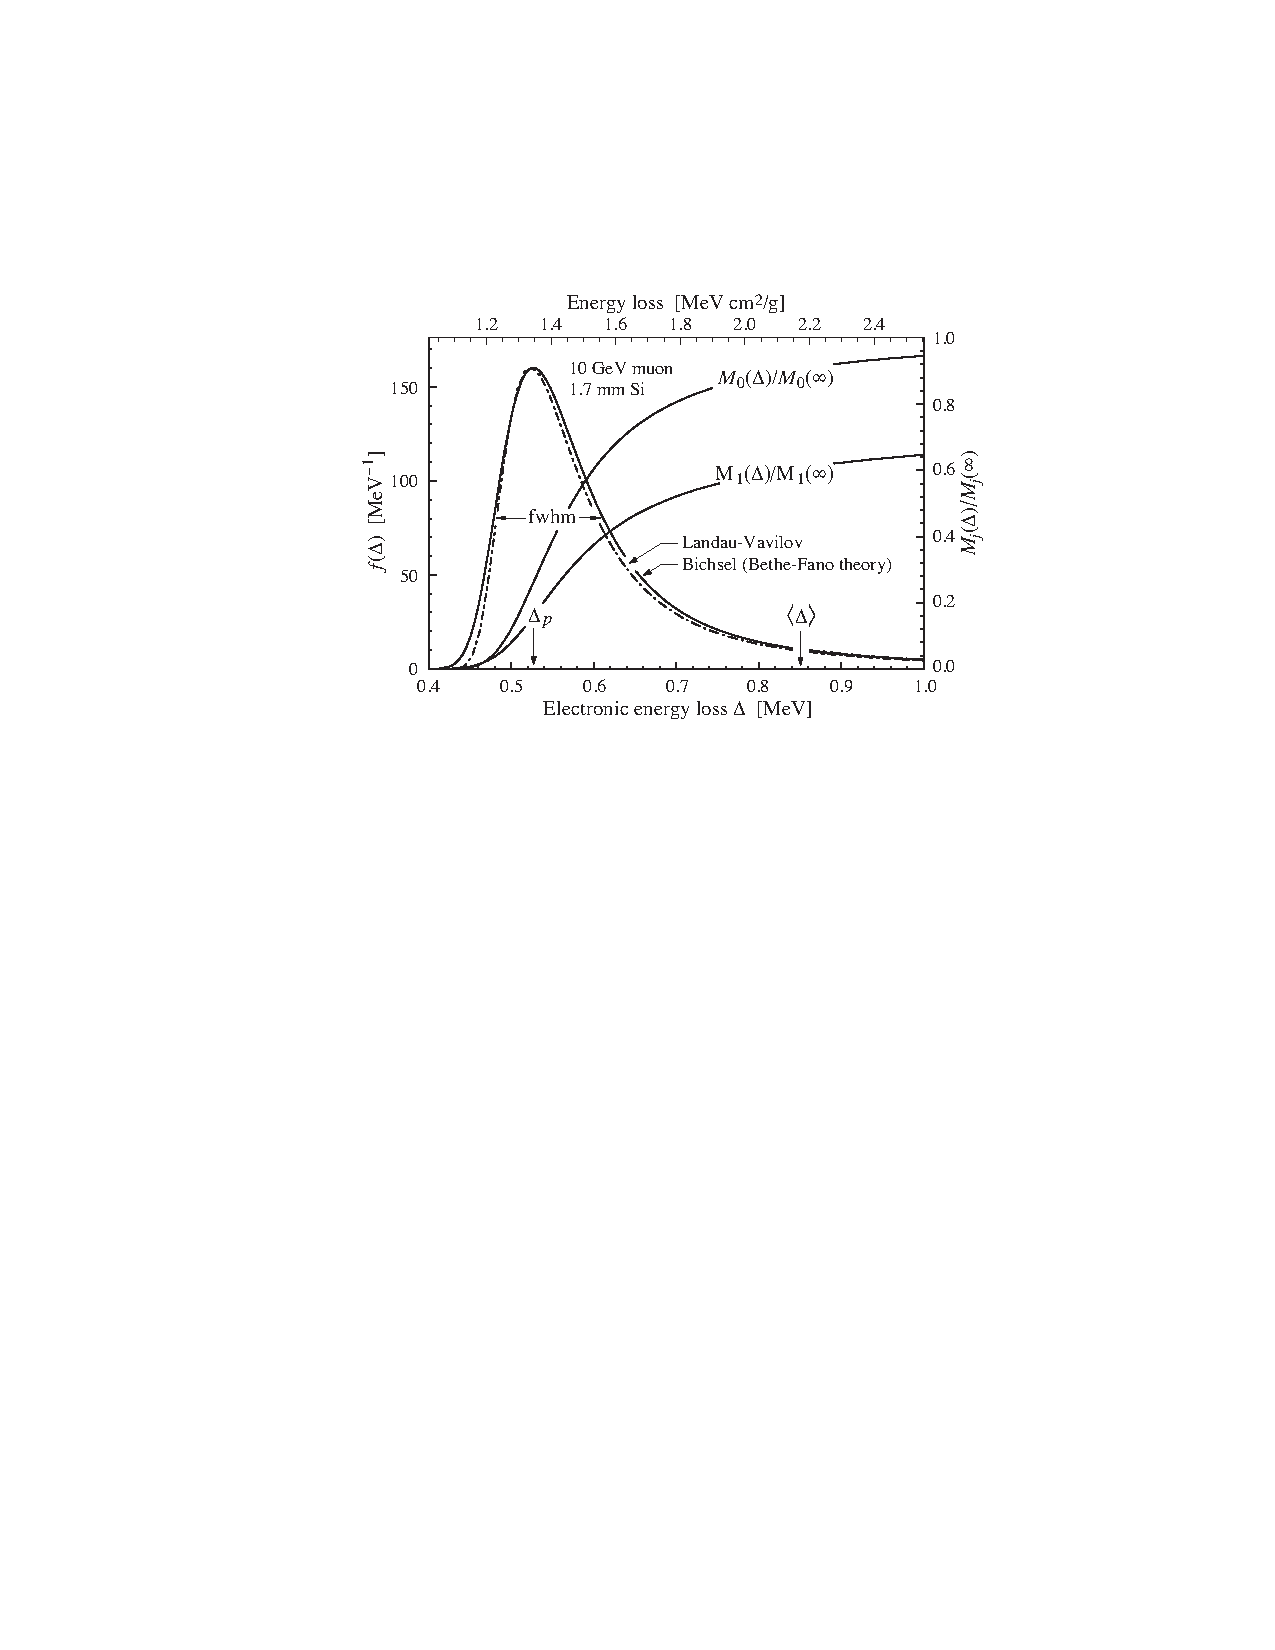
\includegraphics[]{./input/landau.pdf}\caption{Landau-Verteilung des nach Bethe-Bloch berechneten Energieverlusts.\cite{Passage_through_matter}}\label{fig:landau}
\end{figure}
\subsection{Elektronen und Photonen}
Photonen und Elektronen verlieren ihre Energie in Materie hauptsächlich durch Bremsstrahlung (Elektronen), und Paarerzeugung (Photonen). Weil ein Elektron durch Bremsstrahlung Photonen aussendet und ein Photon durch Paarerzeugung Elektronen erzeugt sind beide Vorgänge eng miteinander verbunden. Eine Materialkonstante, die eine wichtige Rolle spielt ist die Strahlungslänge $X_0$. Sie entspricht der Länge nachdem ein Elektron in Materie alles bis auf $1/e$ seiner Energie abgegeben hat. Gleichzeitig ist es $7/9$ der mittleren freien Weglänge eines Photons in diesem Material. Die aufeinander folgende Bremsstrahlung und Paarerzeugung von Photonen und Elektronen führt zu einer Teilchenkaskade, wie schematisch in Abb. \ref{fig:teilchen_kaskade} dargestellt.
\begin{figure}
\centering
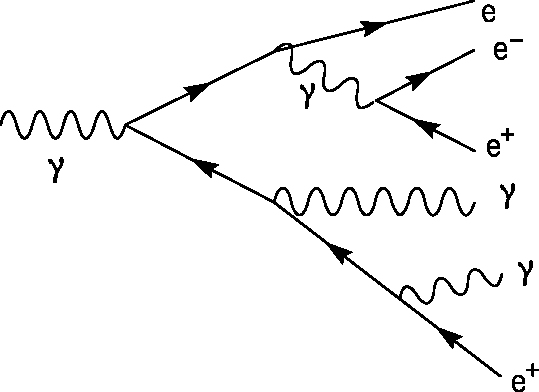
\includegraphics[]{./input/Schematic_of_a_particle_shower.pdf}\caption{Schematische Darstellung einer Elektromagnetischen Kaskade auch Schauer genannt\cite{emKaskade}.\comment{Wikipedia}}
\end{figure}

\section{Gas-Detektoren}
\subsection{Geiger-Zähler}
\subsection{Driftkammer}
\subsection{Time-Projection-Chamber}
text
\section{Teilchen Identifikation}
\subsection{Energieverlust}
\subsection{Time of Flight}
\subsection{Cherenkov Strahlung}
\subsection{Übergangsstrahlung}
text
\section{Cherenkov Detektoren}
text
\section{Halbleiter Detektoren}
\subsection{Halbleiter}
\subsection{Strahlungsschäden}
\subsection{Signalerzeugung}
\subsection{Silizium Detektor}
text
\section{Kalorimeter}
\subsection{Elektromagnetische Schauer}
\subsection{Hadronische Schauer}
\subsection{Sampling und homogene Kalorimeter}
\subsection{Energieauflösung}
text

\chapter{Werkzeuge}
\section{Werkzeuge}

\section{ROOT Data Analysis Framework}

\section{Grid-Computing}

\chapter{Ergebnisse}
\chapter{Diskussion}
\chapter{Zusammenfassung}

\appendix
\chapter{Anhang}


\cleardoublepage
%% Bibliographie. Das Argument muss der Name der BIBTeX-Datenbank stehen.
%% Ein Beispiel fuer eine solche Datenbank finden Sie in bthesis_datenbank.bib
\bibliography{bthesis_datenbank} 


%% Dieser Befehl MUSS am Ende stehen und erzeugt die Erklaerung ueber die
%% benutzten Mittel
%\begin{otherlanguage}{ngerman}
%\Declaration
%\end{otherlanguage}
\end{document}
